\section{Проектирование системы, разработка языка и алгоритма}

\subsection{Архитектура системы}

Рассмотрим архитектуру системы по модели С4~\cite{c4-model}.

\subsubsection{Взаимодействие систем}

В схеме архитектуры на уровне контекста можно наблюдать взаимодействие различных систем, а также взаимодействие этих систем с пользователями и специалистами. Схема взаимодействия представлена на рисунке \ref{System Context}.

\begin{figure}
  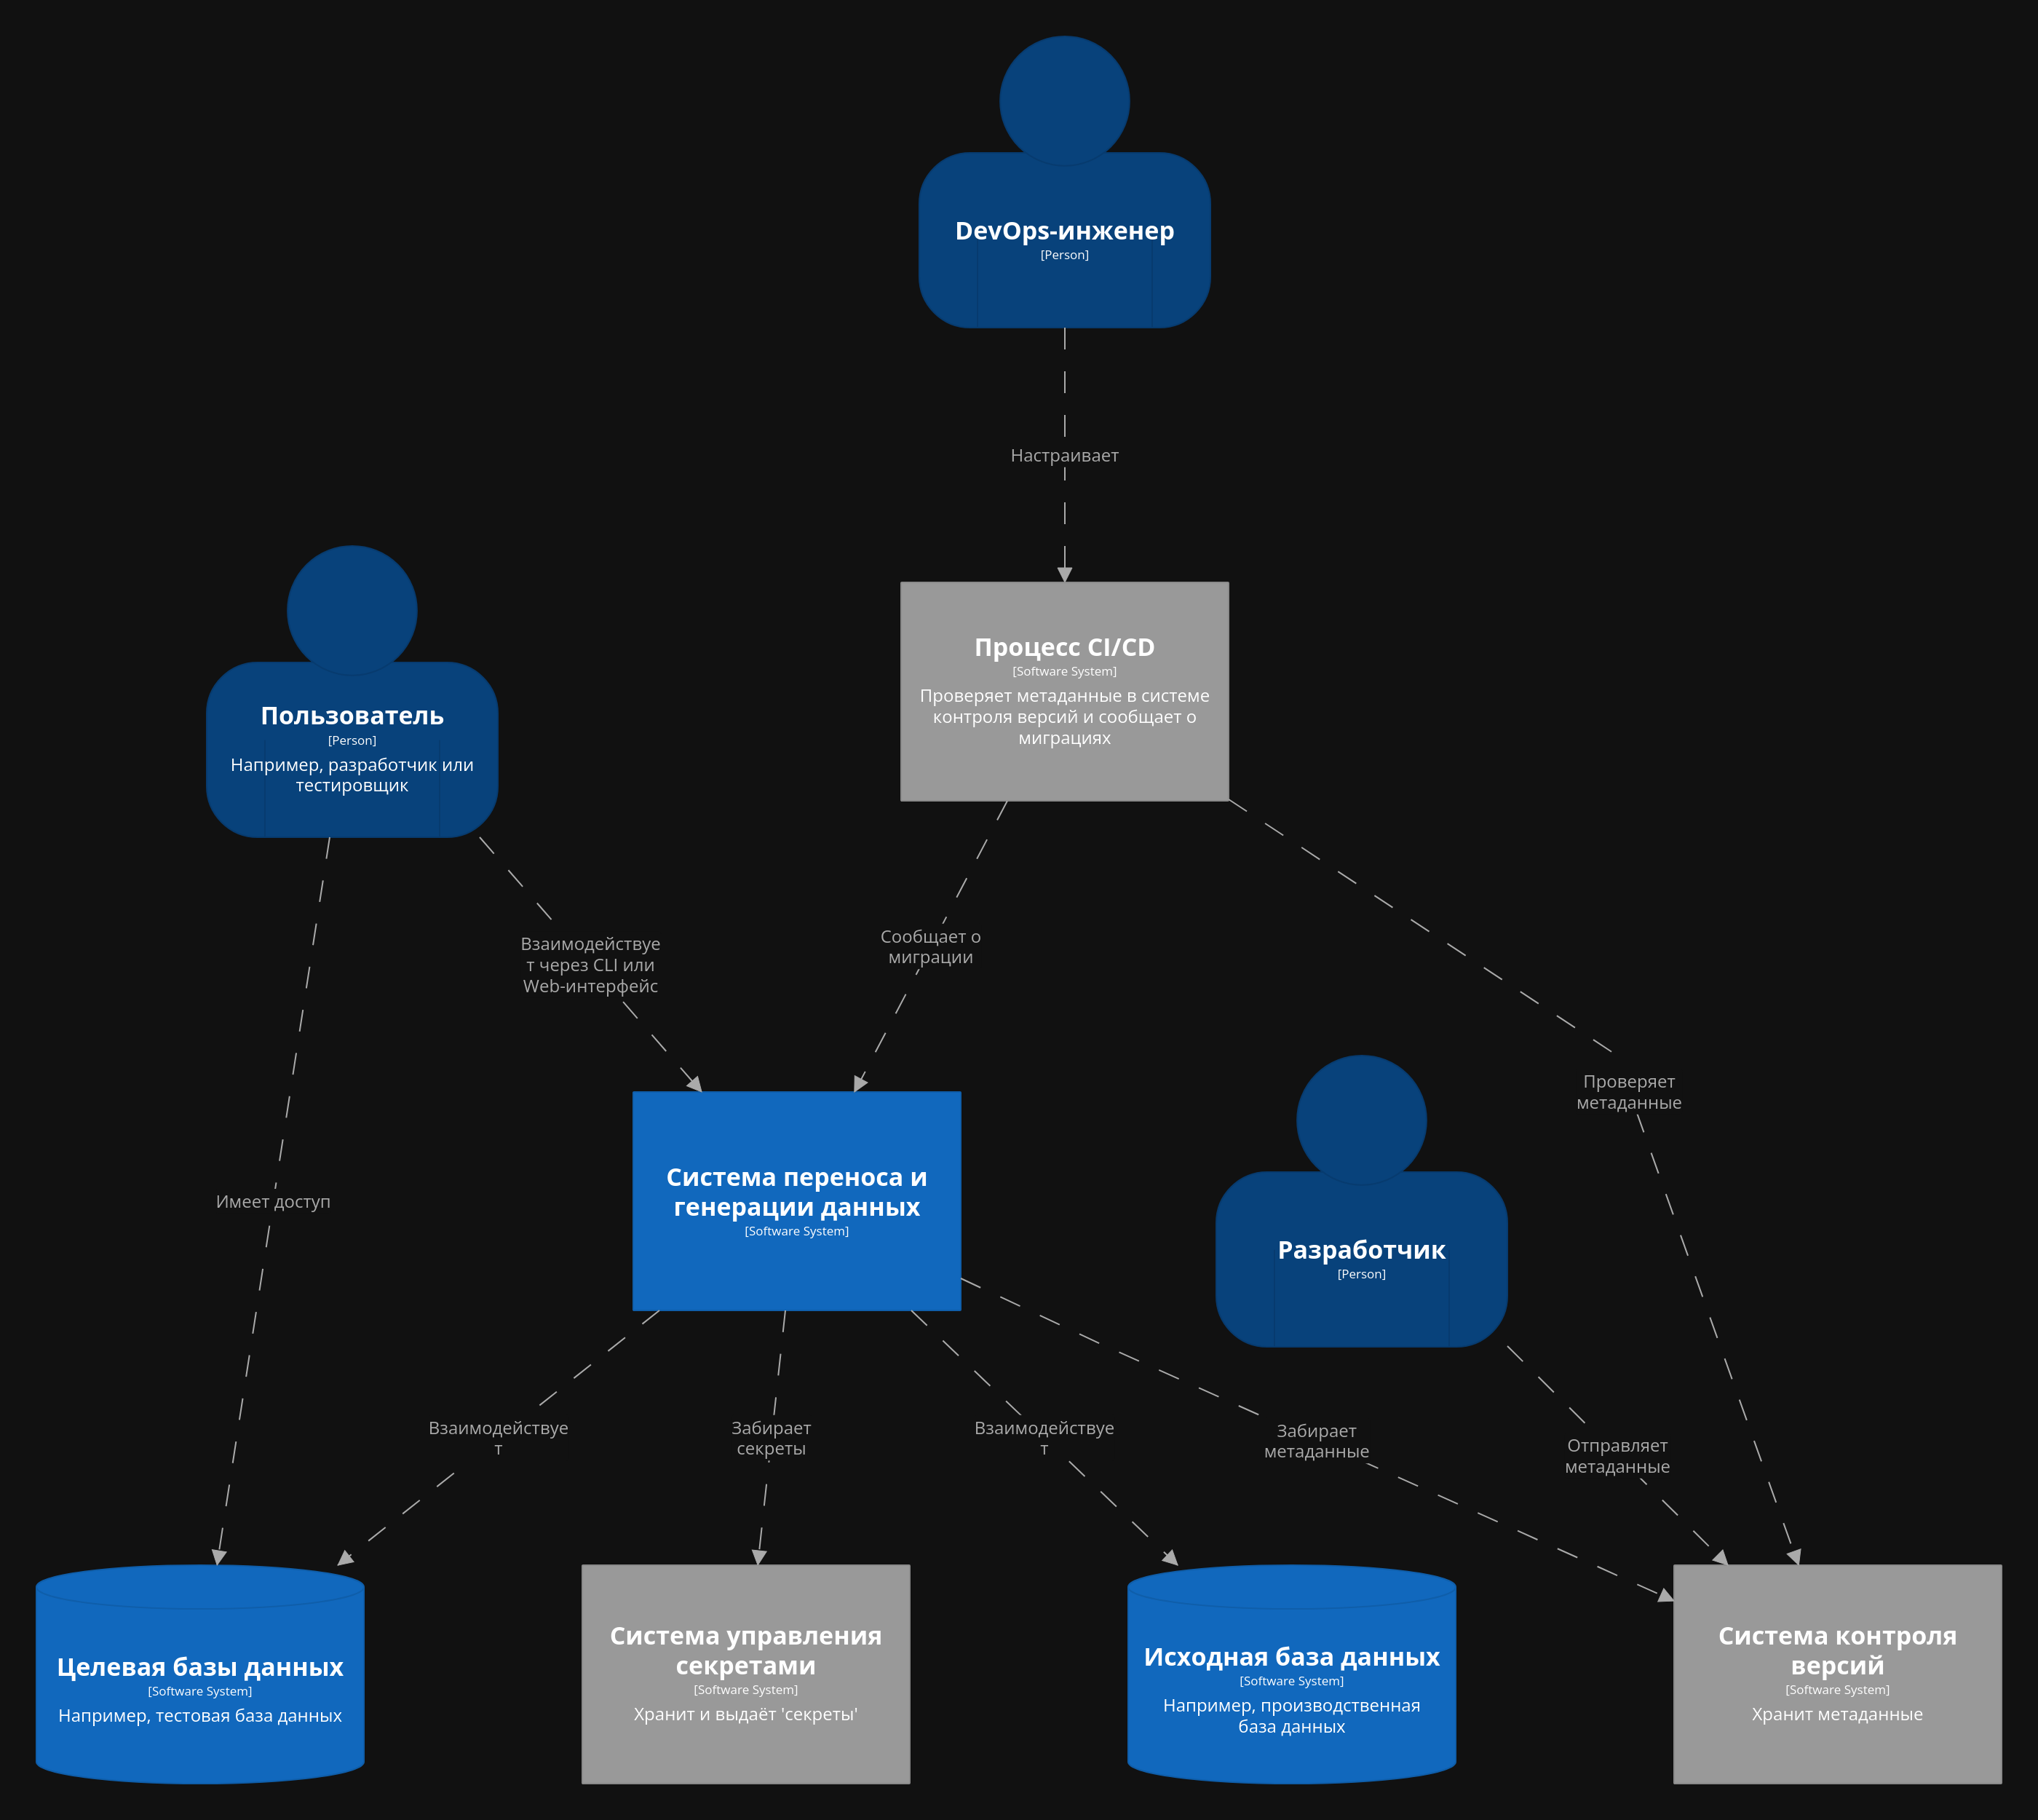
\includegraphics[scale=0.15]{./img/structurizr-SystemLandscape.png}
  \caption{Взаимодействие систем}
  \label{System Context}
\end{figure}

Внешние системы выделены серым цветом:
\begin{itemize}
\item система контроля версий выступает в качестве хранилища метаданных, представленных разработчиком;
\item система управления секретами предоставляет данные для подключения к базе данных;
\item процесс CI/CD, который настраивает DevOps-инженер, выполняет несколько функций:
  \begin{itemize}
    \item генерация тестовой среды и запуск автоматизированных тестов при получении запроса на слияние в систему контроля версий;
    \item проверка корректности метаданных в момент их фиксации в системе контроля версий;
    \item при выполнении миграций осуществляется уведомление системы переноса и генерации данных о процессах миграции. Такой механизм необходим для предотвращения неопределенного поведения, которое может возникнуть, если система в текущий момент работает с мигрируемой базой данных.
  \end{itemize}
\end{itemize}

Синим цветом выделены собственные системы: исходная и целевая базы данных, с которыми осуществляется взаимодействие пользователей, а также система переноса и генерации данных, которую мы рассмотрим более детально далее.

\subsubsection{Система переноса и генерации данных}

Рассмотрим систему переноса и генерации данных на уровне контейнеров. Схема контейнеров представлена на рисунке \ref{Containers}.

\begin{figure}
  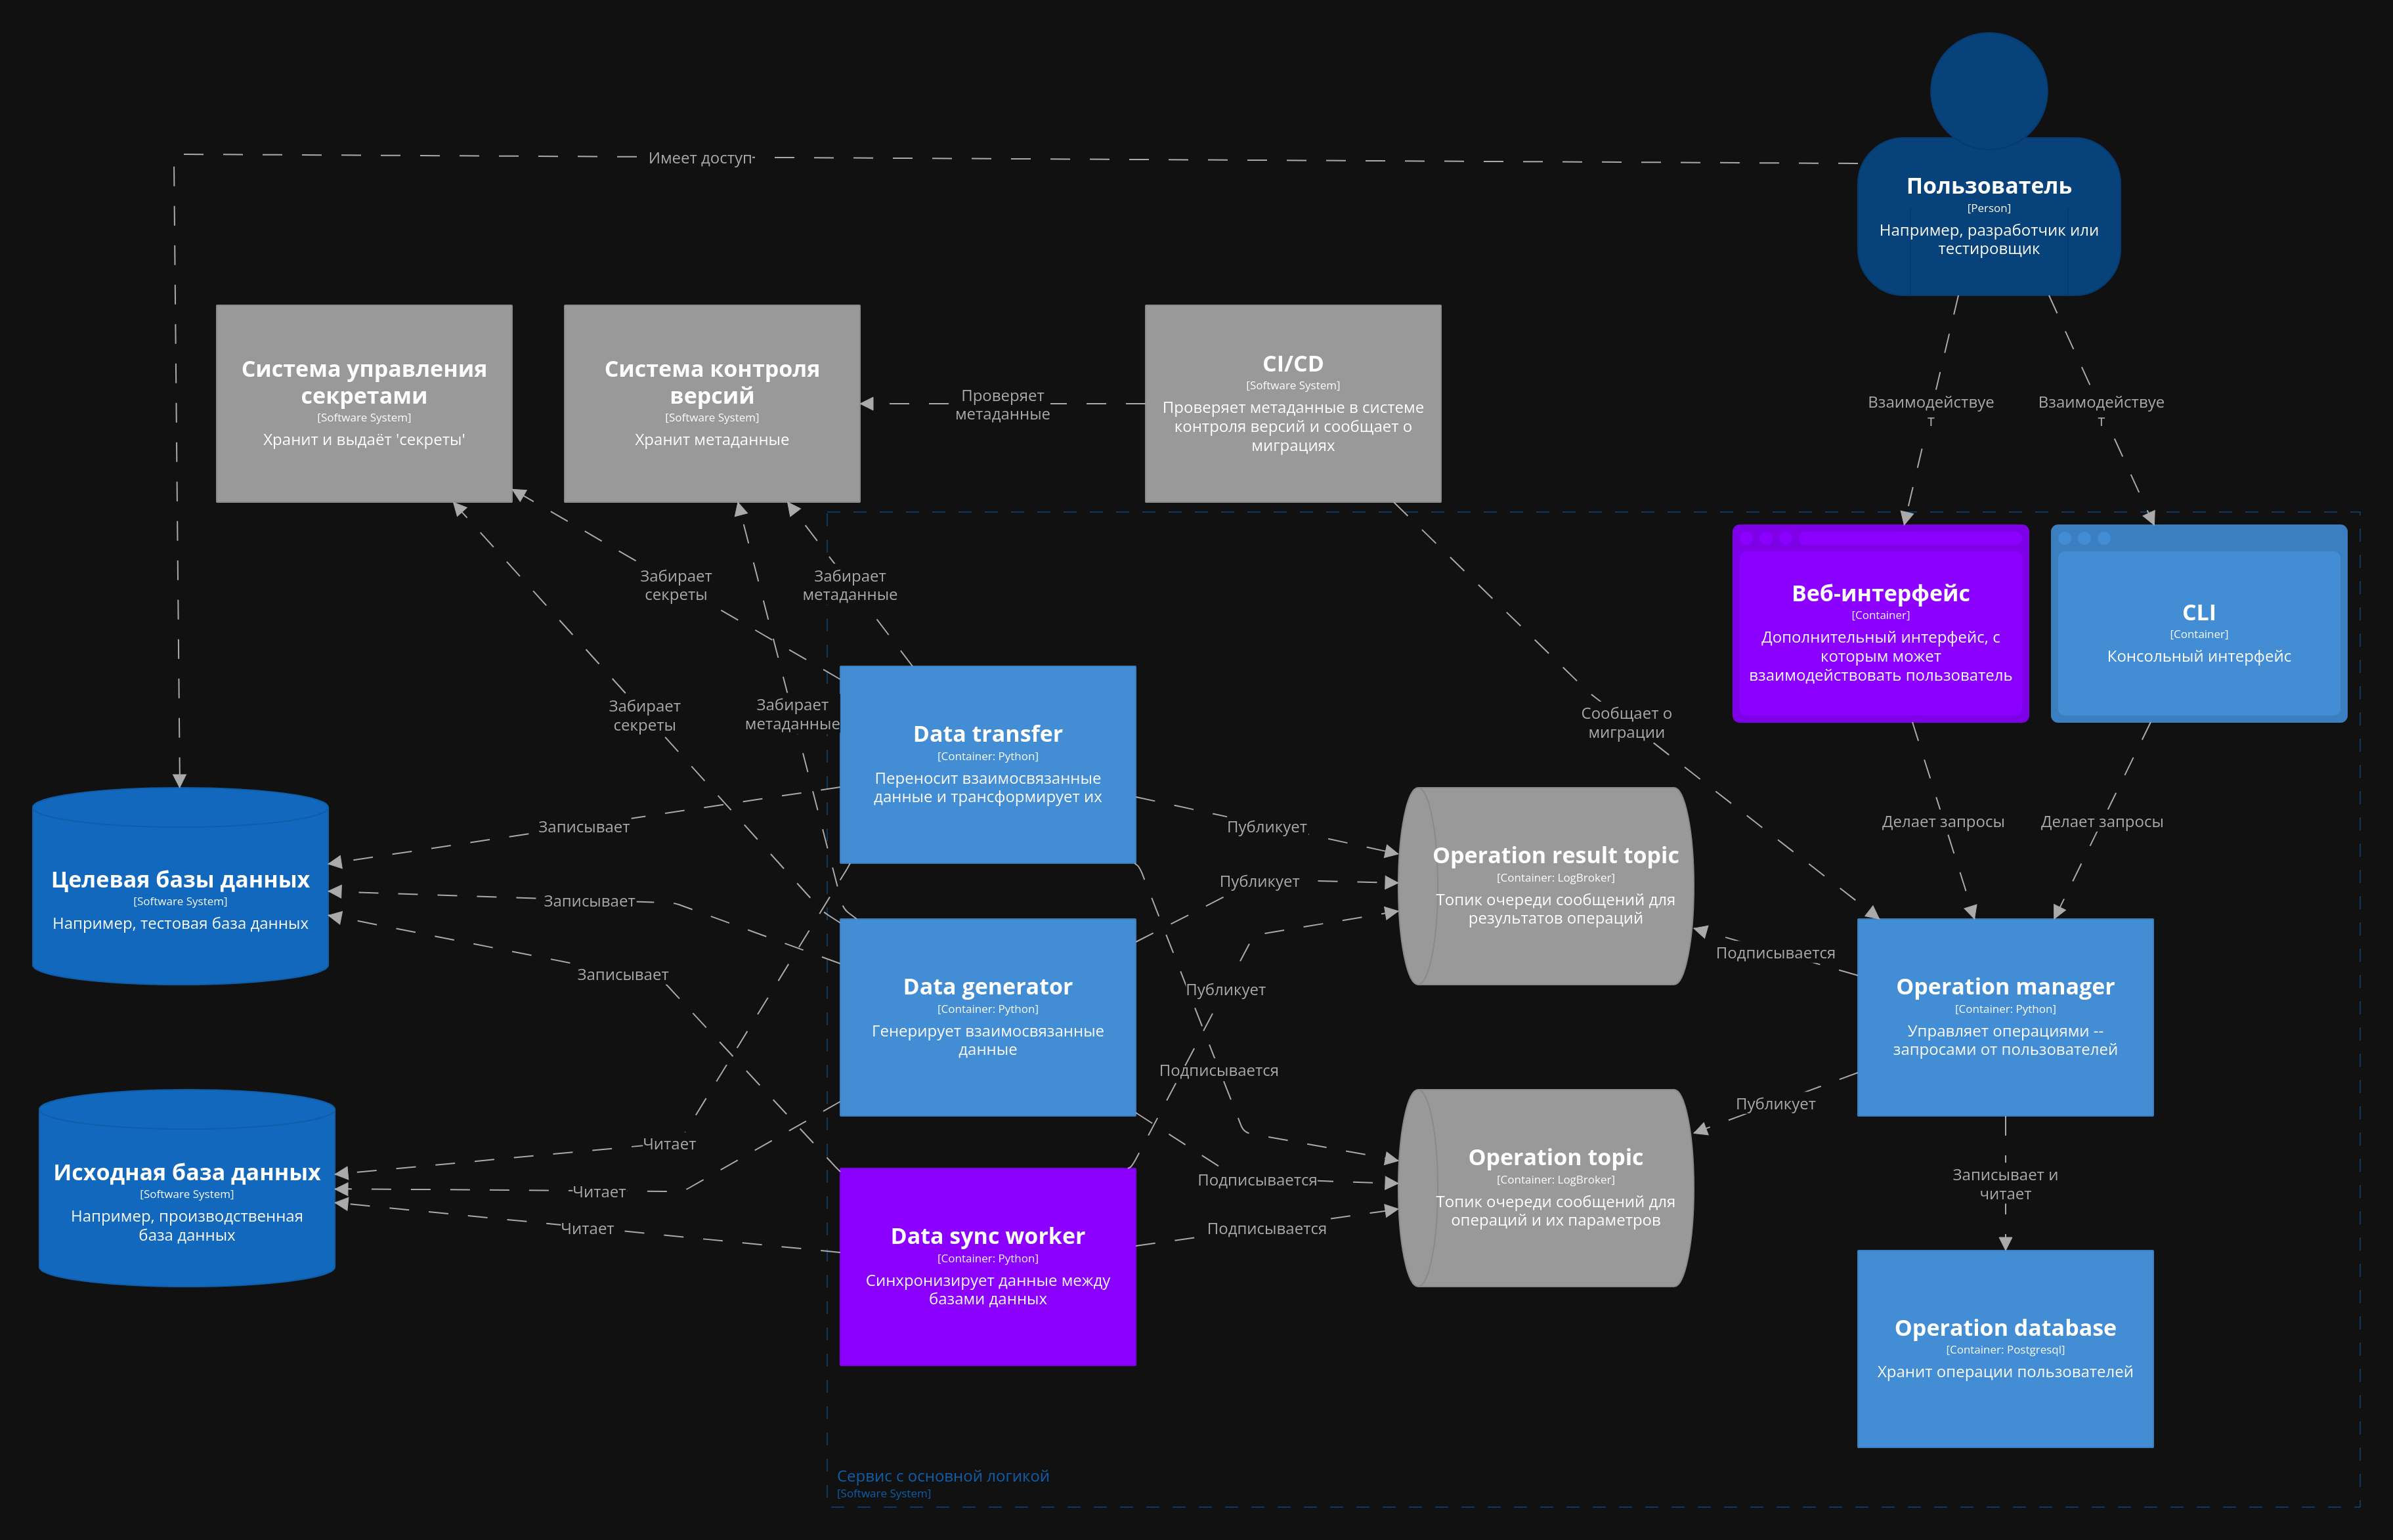
\includegraphics[scale=0.12]{./img/structurizr-Containers.png}
  \caption{Система переноса и генерации данных}
  \label{Containers}
\end{figure}

Взаимодействие пользователя с системой осуществляется через командную строку (CLI), хотя может быть реализован и альтернативный интерфейс взаимодействия, например, веб-интерфейс (выделен фиолетовым как контейнер, который может быть добавлен в перспективе).

Пользователь посылает запросы в контейнер Operation Manager. Возможны два типа запросов: запуск операции по переносу или генерации данных, а также проверка статуса выполняемой операции. В случае получения запроса на запуск операции, информация об операции сохраняется в базе данных, а уникальный идентификатор операции возвращается пользователю, что позволяет ему отслеживать статус выполнения.

Далее Operation Manager отправляет запросы на выполнение операции в очередь сообщений Logbroker~\cite{logbroker}. Контейнер, обрабатывающий такой запрос, определяется типом операции: если речь идет о переносе данных, операция обрабатывается контейнером Data Transfer; если о генерации данных — контейнером Data Generator.

На схеме также представлен контейнер Data Sync Worker, предназначенным для обработки операций по синхронизации данных в базах данных. Более подробно этот контейнер в данной работе рассмотрен не будет.

Контейнеры Data Transfer и Data Generator осуществляют перенос и генерацию данных, взаимодействуя с базами данных, системой контроля версий и системой управления секретами. В процессе выполнения операции, а также после её выполнения, информация о статусе возвращается в очередь сообщений, из которой Operation Manager извлекает данные и обновляет статус операции в базе данных.

Более детальное описание структуры компонентов Data Transfer и Data Generator будет представлено в последующих разделах.

Рассмотрим диаграмму последовательности взаимодействия пользователя с системой на примере генерации данных. Диаграмма представлена на рисунке \ref{Sequence User-MainSystem}. На диаграмме можно заметить, как клиент и система общаются асинхронно. Это функциональность закрывает требование \textit{асинхронной обработки запросов} системы.

\begin{figure}
  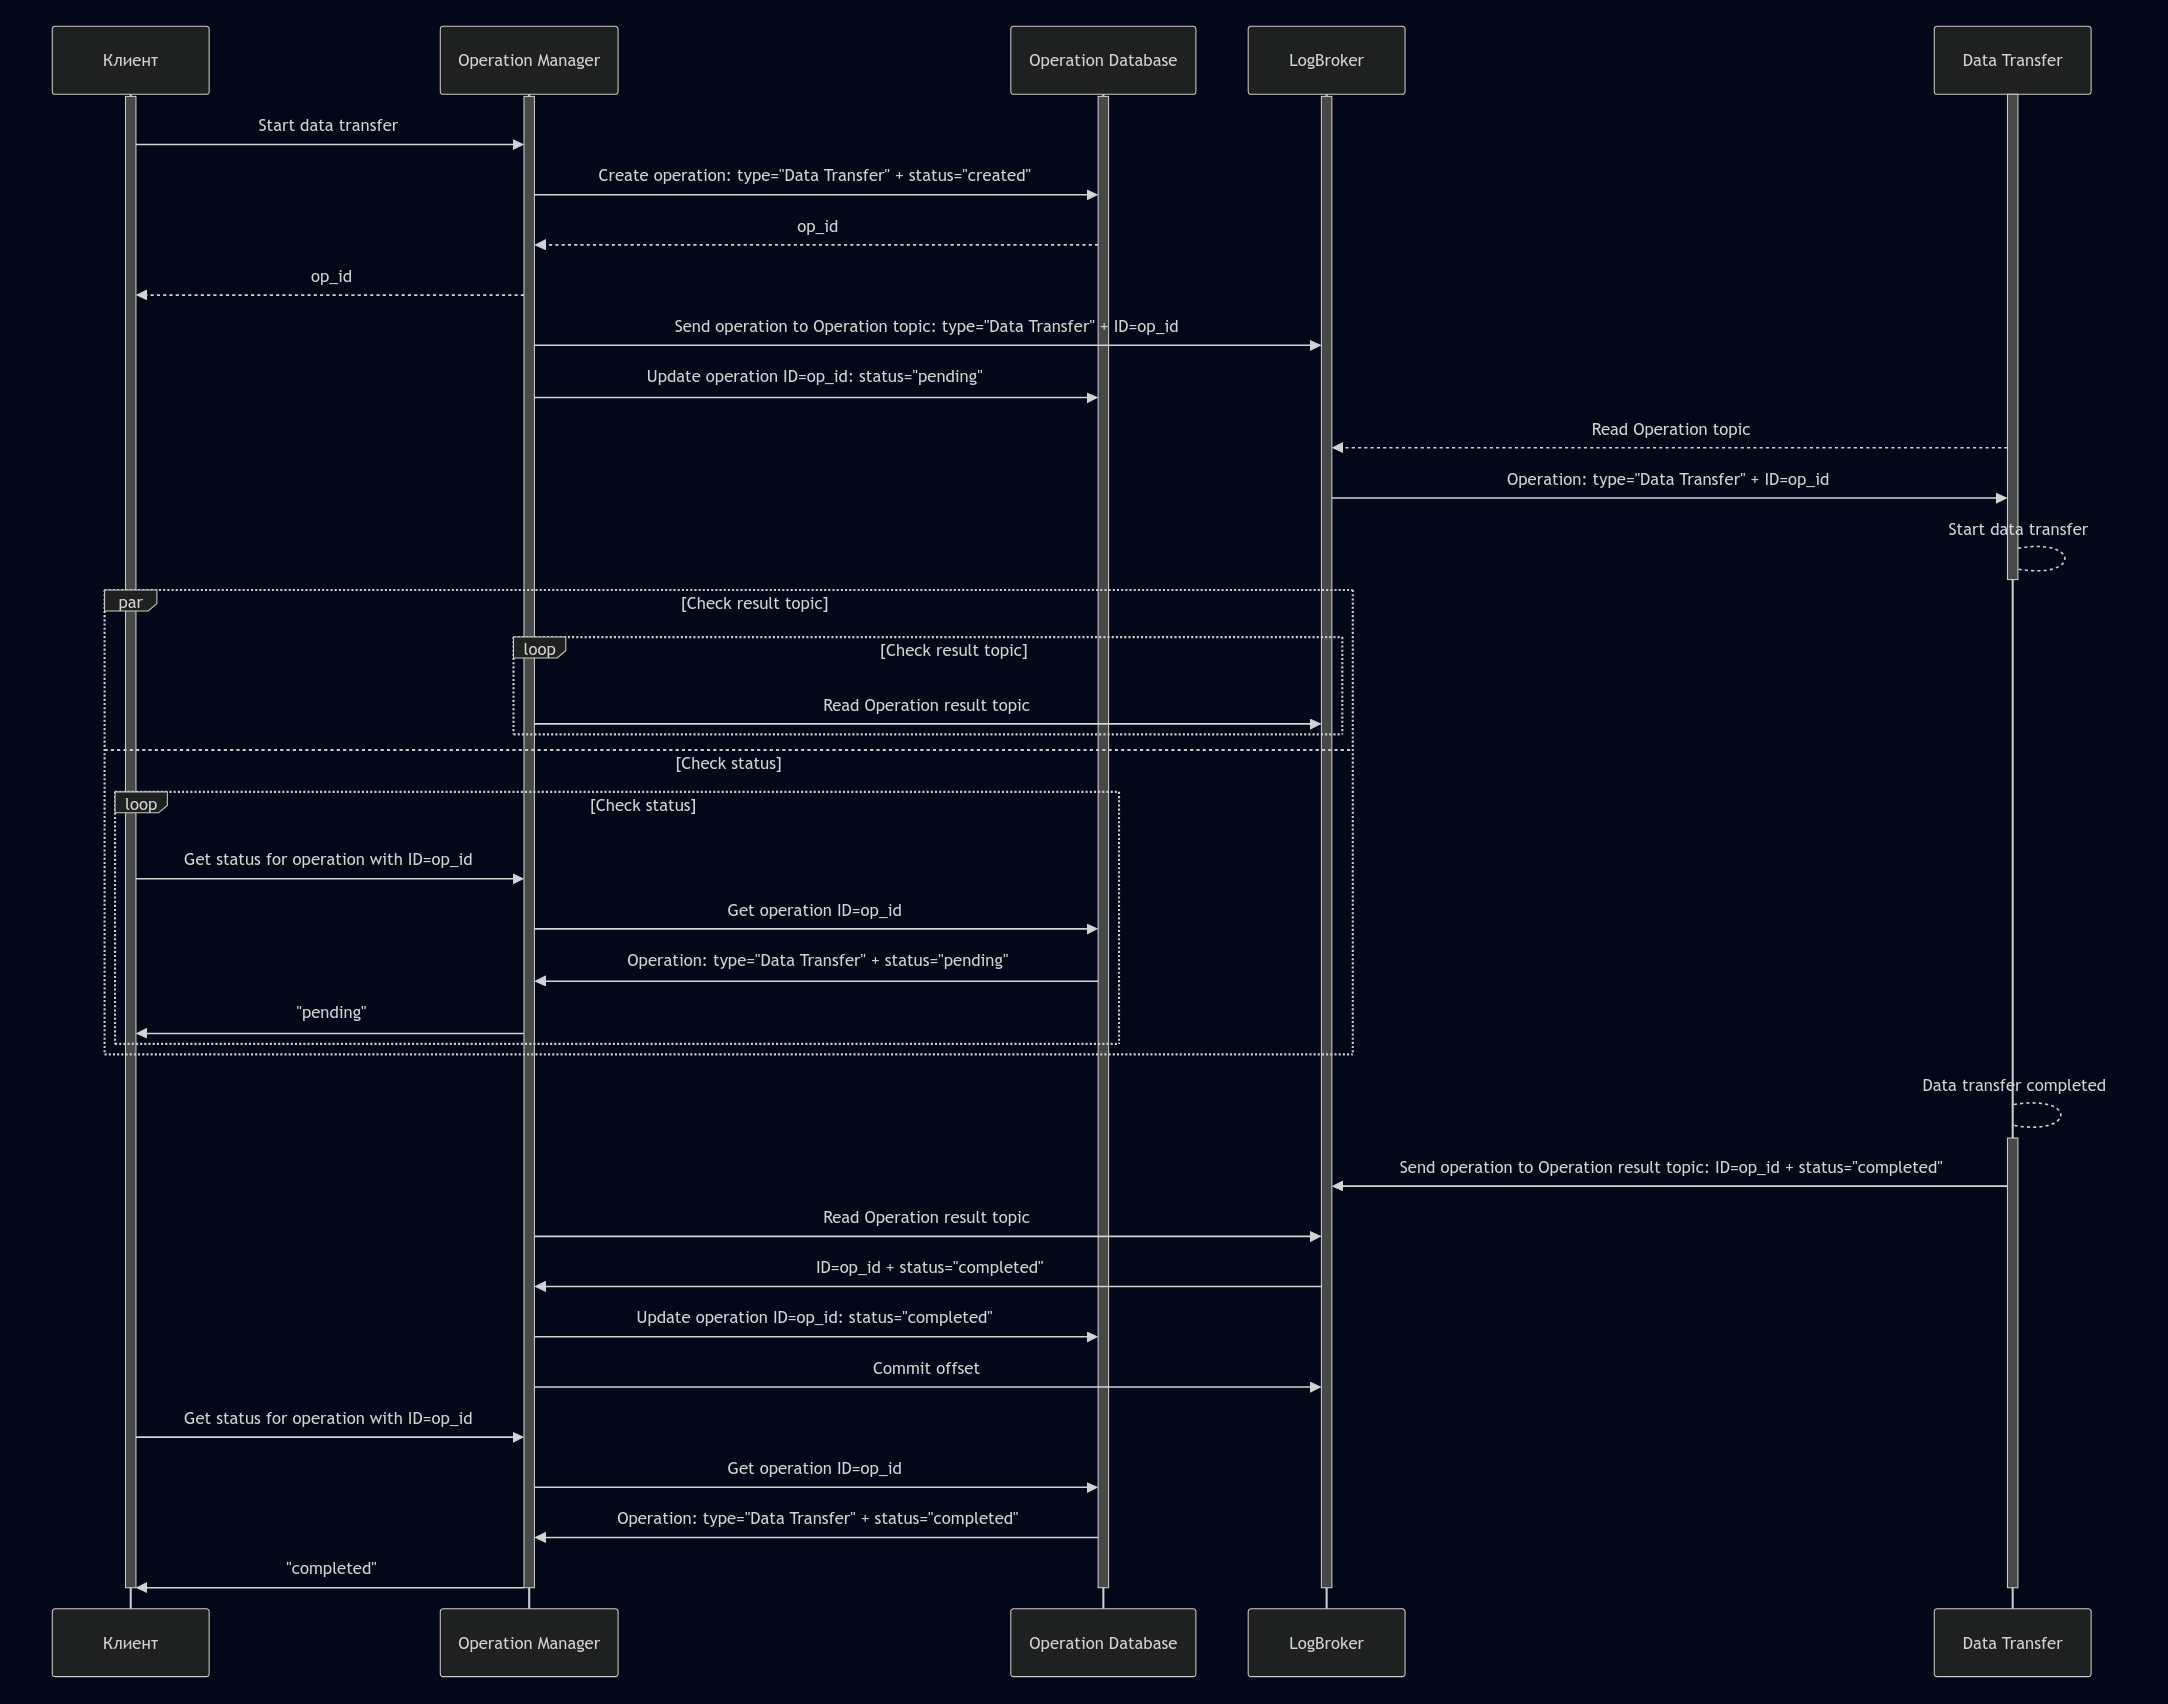
\includegraphics[scale=0.2]{./img/mermaid-sequence-User-MainSystem.png}
  \caption{Диаграмма последовательности взаимодействия пользователя с системой на примере генерации данных}
  \label{Sequence User-MainSystem}
\end{figure}

\subsubsection{Компоненты Data Transfer}

Рассмотрим процесс обработки запросов на перенос задач. Схема компонентов контейнера Data Transfer представлена на рисунке \ref{Data Transfer Components}.

\begin{figure}
  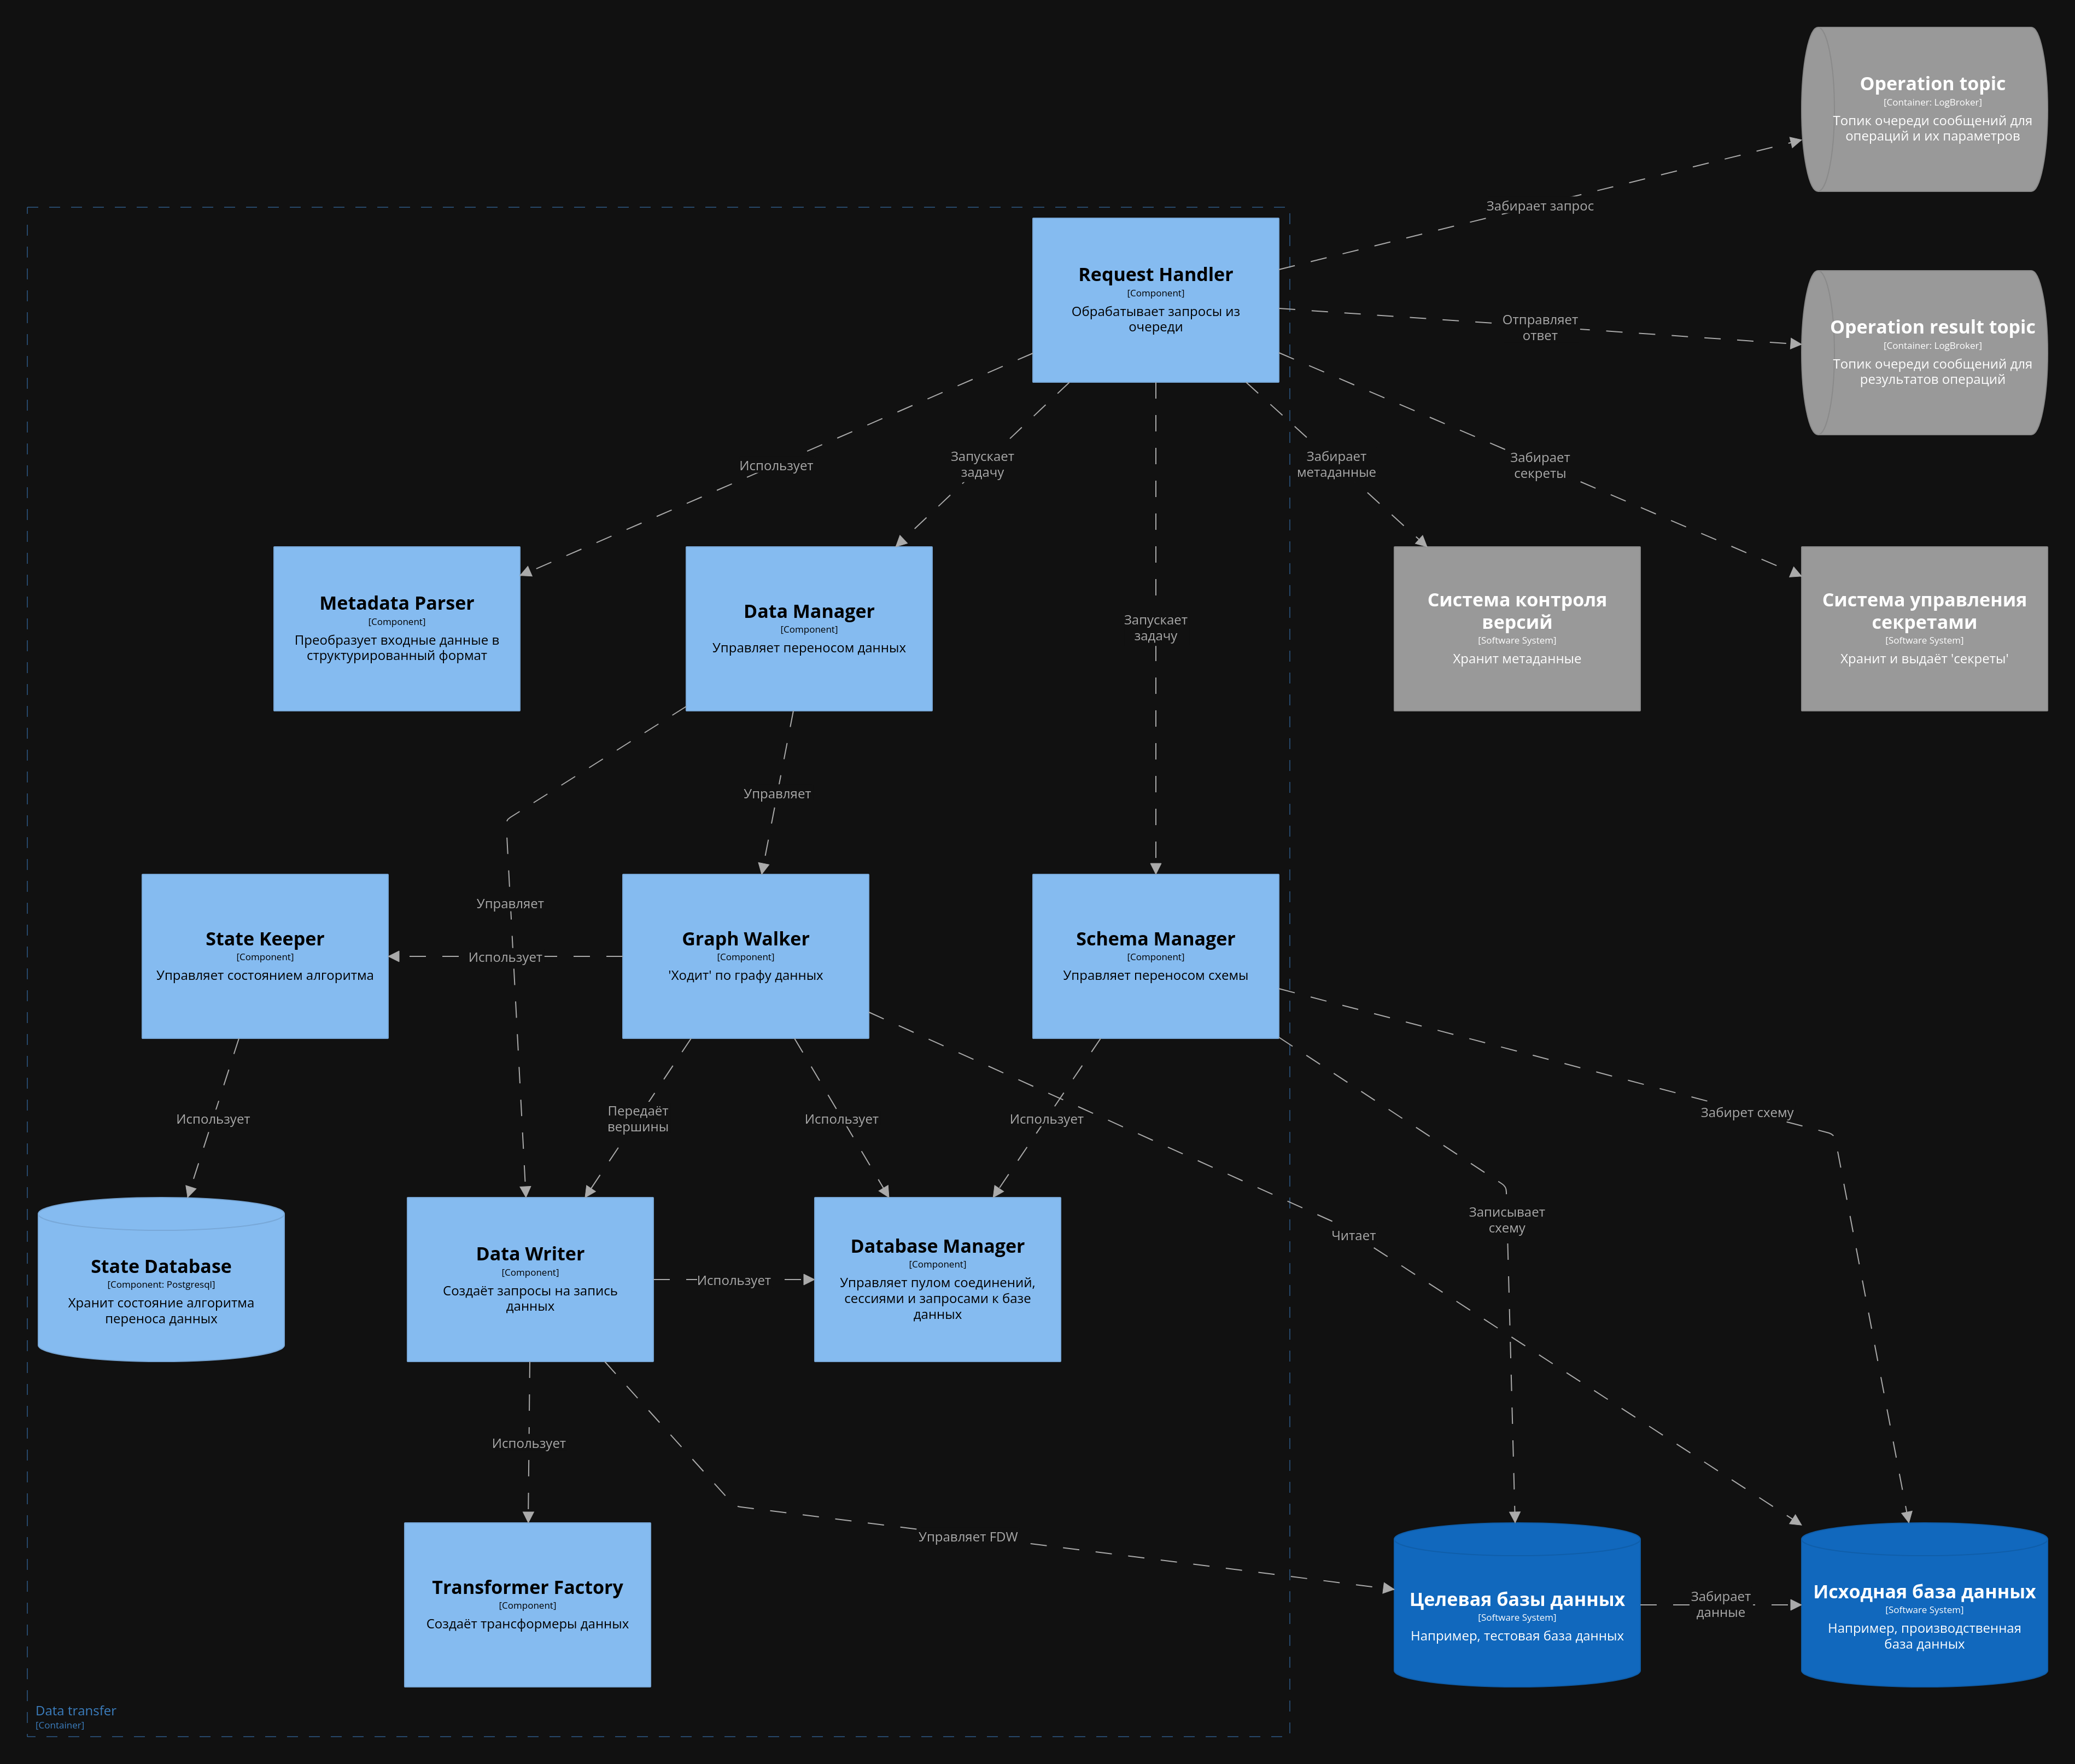
\includegraphics[scale=0.12]{./img/structurizr-DataTransferComponents.png}
  \caption{Компоненты Data Transfer}
  \label{Data Transfer Components}
\end{figure}

Компонент Request Handler принимает такие запросы. Они должны включать следующие элементы:

\begin{itemize}
  \item персональный токен доступа пользователя, который присылает запрос,
  \item идентификатор метаданных,
  \item идентификатор исходной базы данных,
  \item идентификатор целевой базы данных.
\end{itemize}

Идентификатор метаданных может принимать форму одной из двух сущностей: уникального идентификатора, связанного с метаданными в Системе контроля версий, или самих метаданных. В случае предоставления уникального идентификатора, Request Handler обращается к Системе контроля версий для извлечения соответствующих метаданных.

Request Handler осуществляет процедуру верификации прав доступа путем сопоставления идентификаторов баз данных с персональным токеном доступа пользователя, инициировавшего запрос \cite{oauth}. В процессе верификации производится проверка полномочий доступа к исходной и целевой базам данных. В случае отсутствия разрешений у пользователя, дальнейшая обработка запроса прекращается. Такой механизм закрывает требование \textit{безопасности} системы.

Идентификатор базы данных может быть представлен либо в форме уникального идентификатора кластера базы данных, либо в виде параметров подключения к базе данных. При предоставлении уникального идентификатора кластера базы данных, Request Handler обращается к Системе управления секретами для получения параметров подключения, включая пароль.

Полученные метаданные направляются в компонент Metadata Parser для их валидации и преобразования во внутренний формат представления. Далее инициируется Data Manager, который получает информацию о подключениях к базам данных, а также внутреннее представление метаданных, и запускает компоненты Graph Walker и Data Writer.

Компонент Graph Walker выполняет алгоритм обхода данных исходной базы, который будет рассмотрен позже, следуя инструкциям, заданным в метаданных. Он использует State Keeper для сохранения состояния алгоритма и Database Manager для выполнения операций с базой данных. В процессе работы, Graph Walker извлекает метаинформацию о посещенных вершинах и асинхронно передает её компоненту Data Writer.

Компонент Data Writer управляет преобразованием данных и их записью в целевую базу данных. Он принимает на вход метаинформацию о данных, включая их идентификаторы, и с помощью Database Manager создаёт объект Foreign Data Writer~\cite{fdw} в целевой СУБД, обеспечивая прямое подключение к исходной СУБД. Data Writer формирует запросы, включающие идентификаторы данных, направляя их в целевую СУБД для извлечения конкретных данных из исходной базы. Запросы дополняются трансформерами, сформированными на основе метаданных через компонент Transformer Factory. Трансформер представляет собой набор правил преобразования данных, предназначенных для анонимизации данных.

Рассмотрим взаимодействие основных компонент на диаграмме последовательности, представленной на рисунке \ref{Sequence DataTransferComponents}.

\begin{figure}
  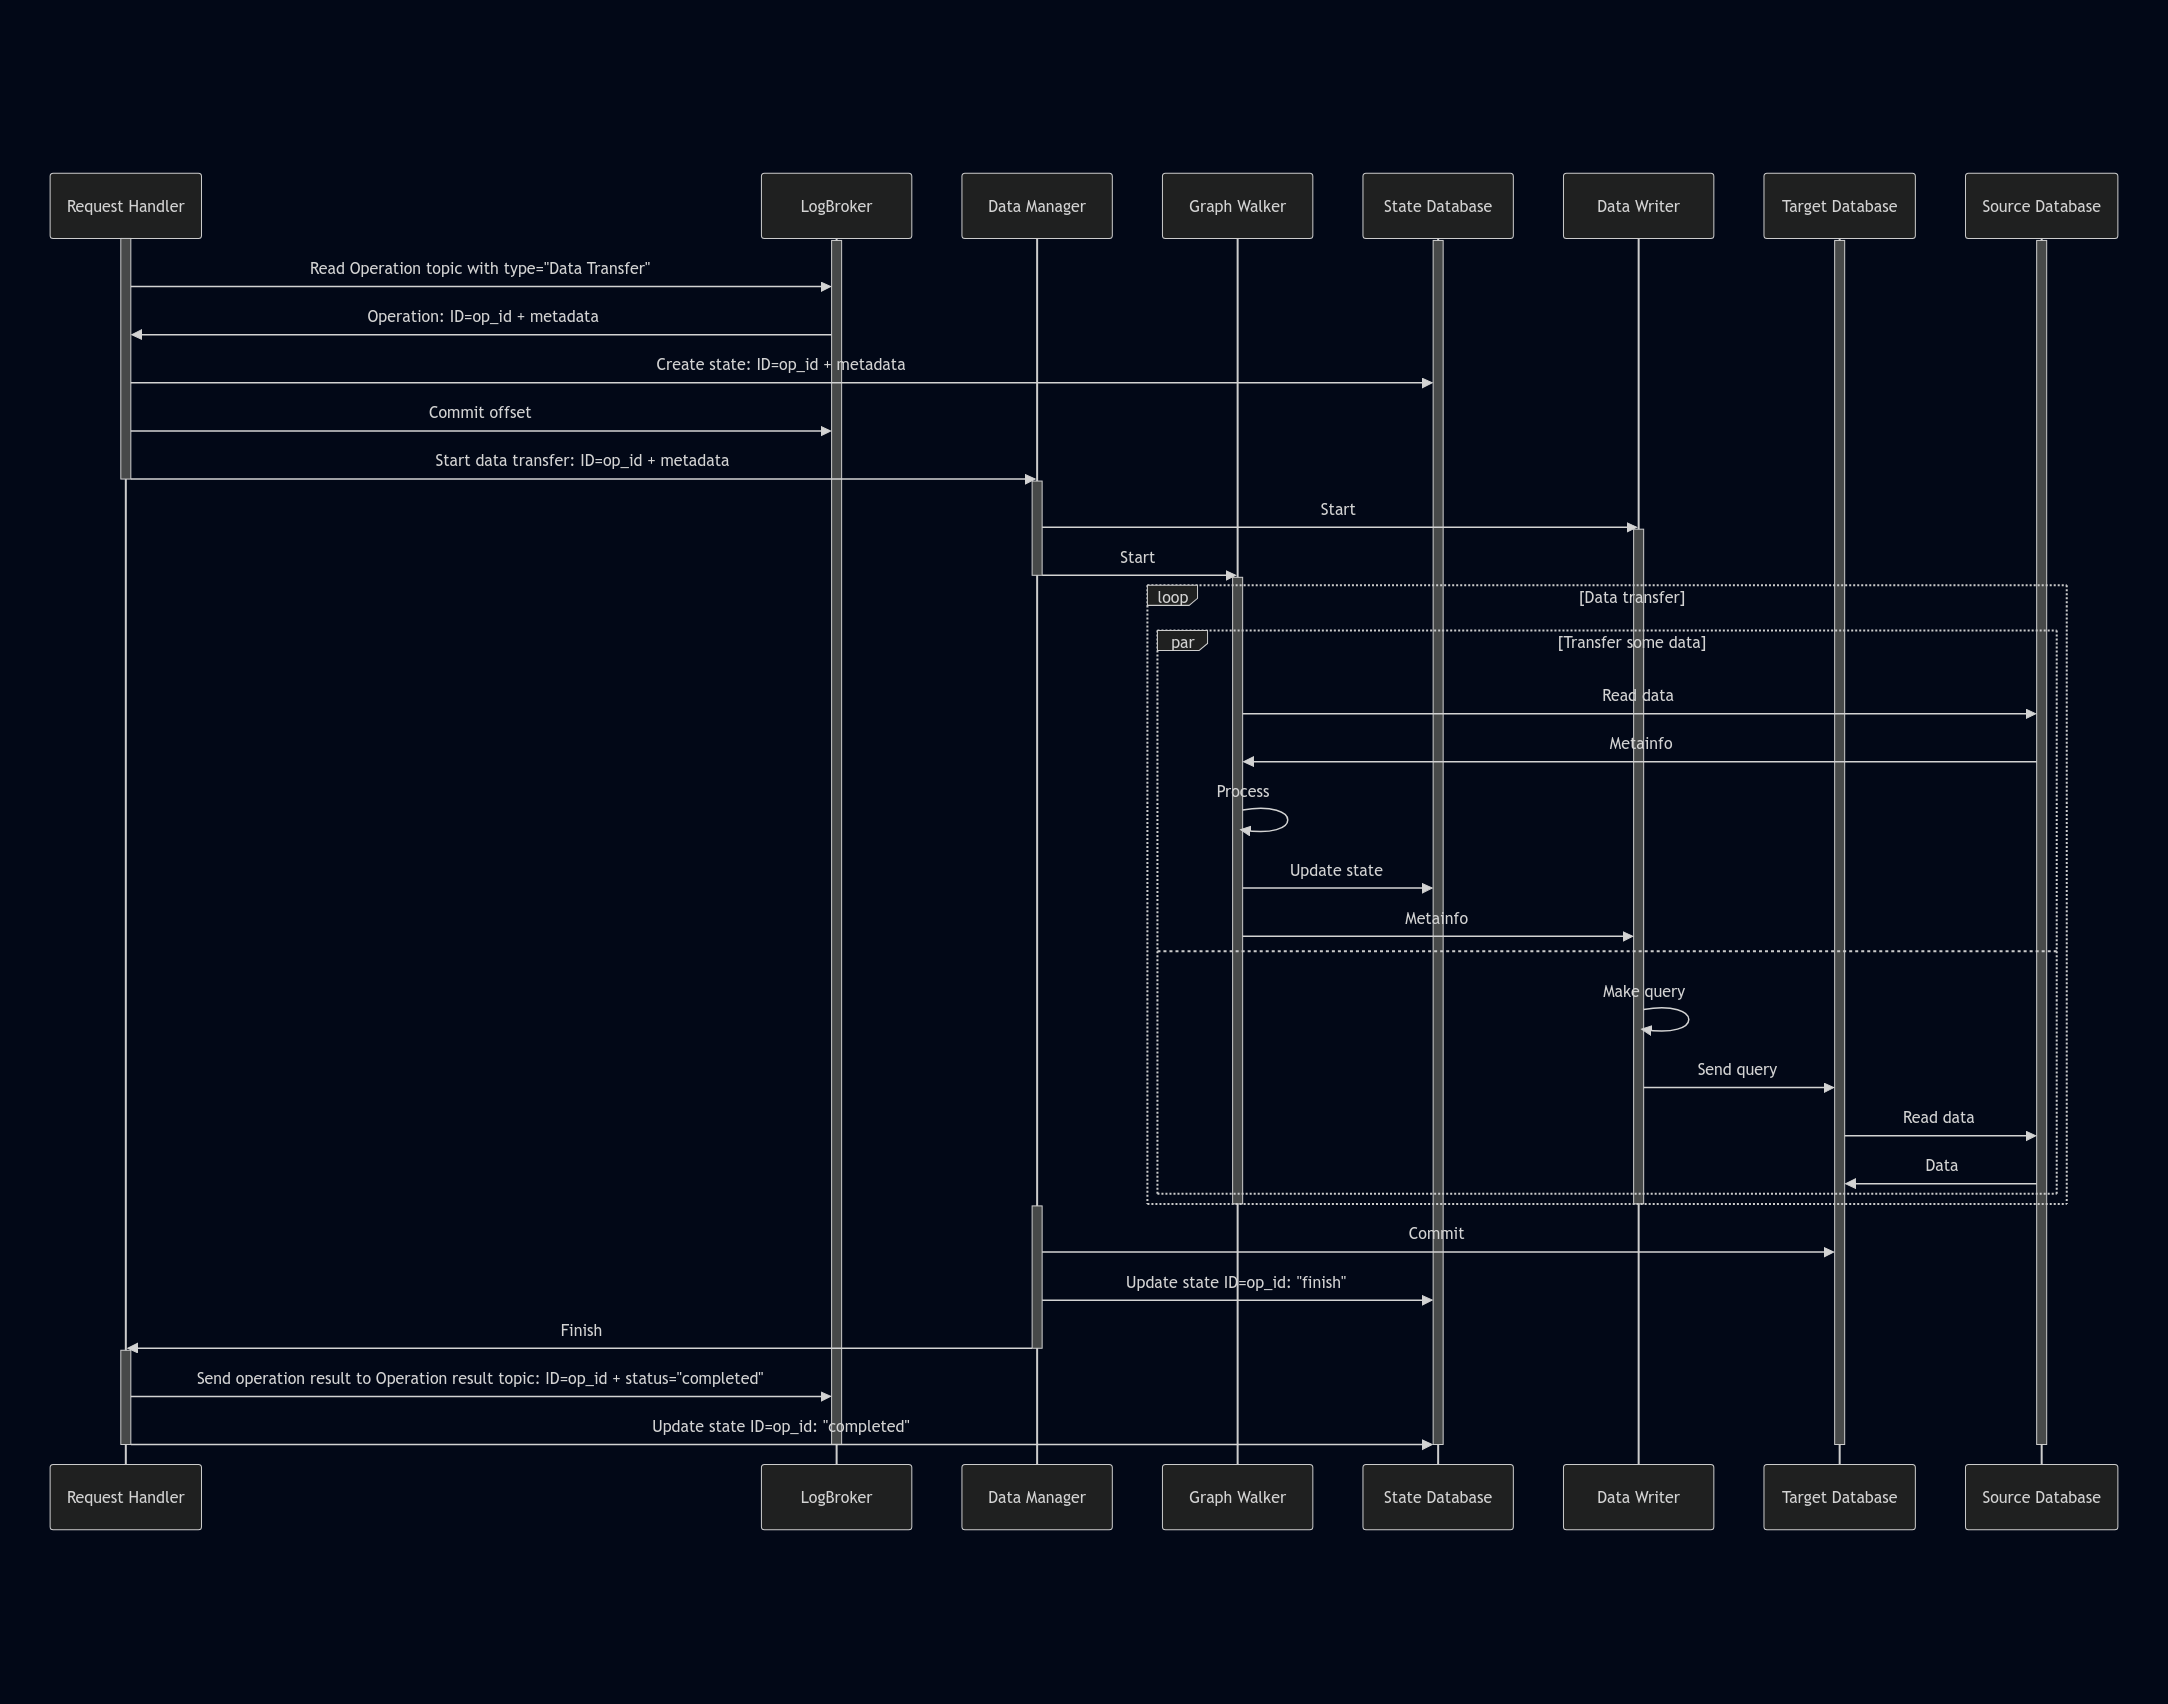
\includegraphics[scale=0.2]{./img/mermaid-sequence-DataTransfer.png}
  \caption{Диаграмма последовательности взаимодействия пользователя с системой на примере генерации данных}
  \label{Sequence DataTransferComponents}
\end{figure}

Данный подход предусматривает непосредственный перенос данных из исходной базы в целевую, с возможными изменениями в соответствии с правилами, определёнными в метаданных, что способствует повышению \textit{производительности} системы.

Также на рисунке~\ref{Data Transfer Components} представлен компонент Schema Manager, который предоставляет функциональность по управлению схемами баз данных. В частности, данный компонент позволяет осуществлять перенос схемы между различными базами данных и выполнять удаление схемы.

\subsubsection{Персистентность состояния и восстановление после сбоя}

Процессы переноса данных могут быть времязатратными, независимо от объёма данных. В случае неожиданной остановки сервиса переноса и генерации данных, вызванной сбоем, утрата прогресса по переносу данных становится крайне нежелательным исходом.

Рассмотрим, как выполняется персистентность состояния системы, то есть её способность сохранять и восстанавливать своё состояние после остановки.

Весь процесс выполнения операции от её инициации до её завершения можно разделить на два этапа:
\begin{itemize}
  \item отправка и чтение из очереди сообщений,
  \item непосредственный процесс переноса данных.
\end{itemize}

Сбои могут возникать на любом из этих этапов. Для этапа отправки и чтения сообщений из очереди предусмотрена семантика доставки exactly-once \cite{delivery-guarantees}, которая поддерживается использованием архитектурных паттернов Inbox Pattern и Outbox Pattern \cite{outbox-and-inbox}. Эти паттерны, часть реализации которых были отражены на рисунках \ref{Sequence User-MainSystem} и \ref{Sequence DataTransferComponents}, обеспечивают гарантированную доставку сообщений и идемпотентную обработку входящих данных.

При сбое на этапе переноса данных механизмы восстановления включают проверку состояния незавершённых операций в базе данных состояния (State Database). В ней хранится прогресс каждой операции переноса данных и включает уникальные идентификаторы операции, состояние алгоритма и метаданные. При восстановлении система переноса данных проверяет наличие незавершённых операций и продолжает их с того места, где процесс был остановлен. Запись в целевую базу данных успешно завершается только при успешном выполнении алгоритма, что требует повторной записи данных в случае восстановления после сбоя, основываясь на метаинформации из сохранённого состояния.

Таким образом, архитектура системы включает механизмы обеспечения персистентности состояния и восстановления после сбоев, что закрывает требование \textit{надёжности} системы.

\subsection{Алгоритм обхода данных}

Всю функциональность переноса данных можно разделить на две части: запись данных в целевую базу данных, которую рассматривали ранее, и обход исходных данных, алгоритм которого мы рассмотрим подробнее в этом разделе.

\subsubsection{Метаграфы}
На сегодняшний день в научном сообществе не существует общепринятого и устойчивого определения метаграфа. Работа \cite{metagraphs_1} была первым источником, в котором появился термин "метаграф". Эта концепция всё ещё находится в стадии развития и интерпретируется различными исследователями по-разному в зависимости от их специфических задач и целей \cite{metagraphs_2, metagraphs_3, metagraphs_4, metagraphs_5}. В общем смысле, метаграф можно рассматривать как структуру, которая обобщает и расширяет идеи классических графов, чтобы решить более сложные задачи анализа данных.

В данной дипломной работе предлагается собственное определение метаграфа, адаптированное под требования и задачи рассматриваемого алгоритма.

Пусть $MG = \langle V, MV, E, ME \rangle$ -- метаграф, где $V$ -- множество вершин, $MV$ -- множество метавершин, $E$ -- множество рёбер, $ME$ -- множество метарёбер.

$v_i = \{atr_k\}, v_i \in V$, где $v_i$ -- вершина, $atr_k$ -- атрибут.

$mv_i = \langle \{v_j\}, \{atr_k\} \rangle, mv_i \in MV, v_j \in V$, где $mv_i$ -- метавершина, $v_j$ -- вершина, $atr_k$ -- атрибут.

$e_i = \langle v_s, v_e \rangle, e_i \in E, v_s, v_e \in V$, где $e_i$ -- ребро, $v_s$ -- исходная вершина, $v_e$ -- конечная вершина.
$me_i = \langle mv_s, mv_e, \{atr_k\} \rangle, me_i \in ME, mv_s, mv_e \in MV$, где $me_i$ -- метаребро, $mv_s$ -- исходная метавершина, $mv_e$ -- конечная метавершина, $atr_k$ -- атрибут.

Также введём ограничение на множество метавершин: $\forall mv_i, mv_j \in V, i \neq j => \{v_x\}_i \cap \{v_y\}_j = \emptyset$, т.е. каждая вершина не может содержаться в нескольких метавершинах.

Следует отметить, что метаграф может быть \textit{симметричным}. Это означает, что, во-первых, при наличии метаребра, соединяющего одну метавершину с другой, существует и обратное метаребро, соединяющее вторую метавершину с первой; во-вторых, наличие ребра между двумя обычными вершинами также подразумевает существование обратного ребра. Cимметричный метаграф $MG = \langle V, MV, E, ME \rangle$ определяется следующим образом: если $\langle mv_i, mv_j, \{atr_k\} \rangle \in ME$, то также выполняется $\langle mv_j, mv_i, \{atr_k\} \rangle \in ME$, и если $\langle v_i, v_j \rangle \in E$, то также существует $\langle v_j, v_i \rangle \in E$.

\subsubsection{Представление базы данных в виде метаграфа}

Реляционные базы данных традиционно состоят из множества связанных таблиц, каждая из которых содержит структурированные данные. В метаграфе эти элементы могут быть представлены следующим образом.

\begin{itemize}
  \item метавершины. В контексте метаграфа метавершинам соответствуют конкретные таблицы реляционной базы данных. Набор атрибутов метавершины содержат информацию о структуре таблицы, включая её название, идентификатор и набор столбцов;

  \item вершины. Вершины соответствуют записям в таблицах. Каждый набор атрибутов вершины напрямую соответствует набору значений в конкретной записи таблицы;

  \item метарёбра. Метарёбра описывают связи между различными таблицами в базе данных. Эти связи формируются посредством внешних ключей~\cite{foreign-key}, которые указывают на зависимость одной таблицы от другой. Атрибуты метарёбер содержат информацию о полях, которые связаны между таблицами;

  \item рёбра. Рёбра представляют связи между конкретными записями в таблицах и формируются на основании соответствующих метарёбер. Эти рёбра конкретизируют связь на уровне данных, отражая указанные в метарёбрах отношения через конкретные внутренние связи записей, например, через одинаковые или согласованные идентификаторы.
\end{itemize}

Для иллюстрации представления базы данных в виде метаграфа рассмотрим небольшой пример, содержащий пять таблиц по несколько записей в каждой. На рисунке \ref{db-example} представлена схема взаимосвязей между конкретными записями в базе данных. Красные стрелки указывают на то, что записи, из которых исходят стрелки, имеют ссылки на другие записи. Это свидетельствует о наличии в таблице внешнего ключа, ссылающегося на другую таблицу. В свою очередь, зелёные стрелки обозначают противоположную ситуацию: данные, на которые они указывают, являются объектом ссылок со стороны других записей.

\begin{figure}
  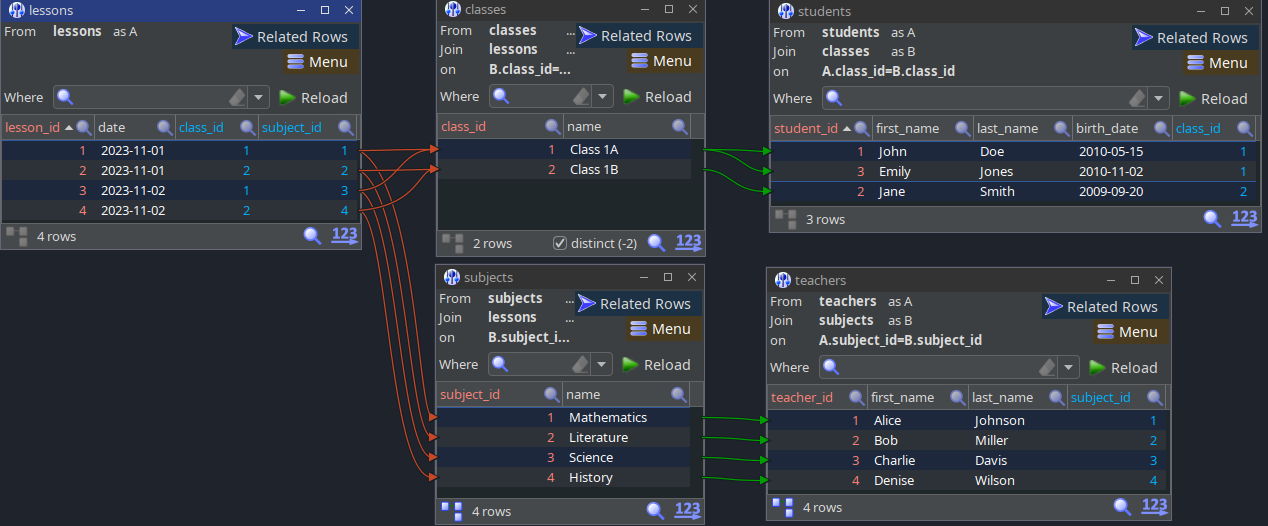
\includegraphics[scale=0.45]{./img/jailer-example-db-overview.png}
  \caption{Пример реляционной базы данных}
  \label{db-example}
\end{figure}

На рисунке \ref{metagraph-example} представлено графическое изображение метаграфа, соответствующего заданной базе данных. Оранжевым цветом обозначены метавершины и метарёбра, которые соответствуют таблицам и связям между этими таблицами. В свою очередь, синим цветом представлены вершины и рёбра, отражающие записи и связи между ними.

\begin{figure}
  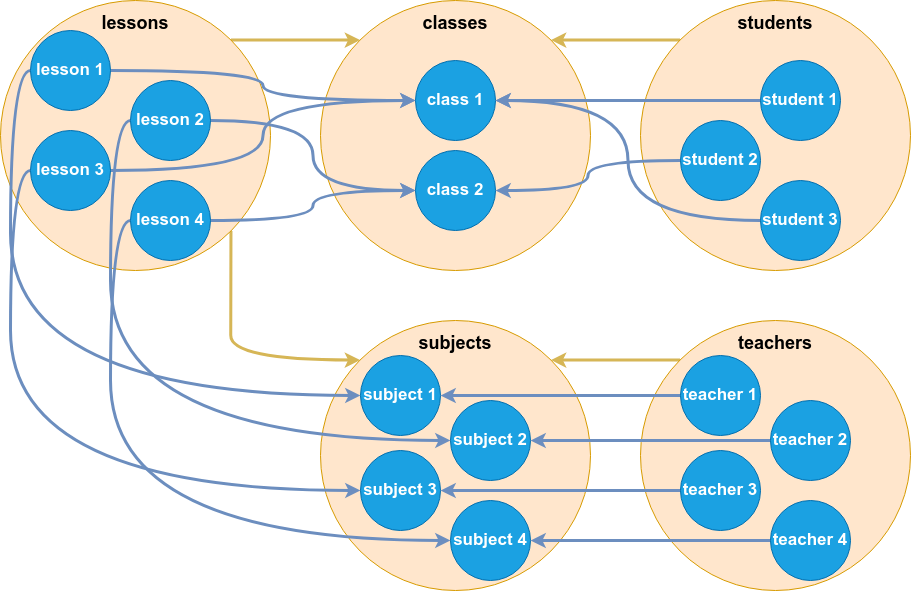
\includegraphics[scale=0.5]{./img/drawio-metagraph-overview.png}
  \caption{Пример метаграфа}
  \label{metagraph-example}
\end{figure}

Далее, для краткости, такой метаграф будем называть \textit{метаграфом базы данных}.

\subsubsection{Описание алгоритма с метаграфом базы данных}
Поскольку теперь можно представить базу данных в виде метаграфа, алгоритм обхода взаимосвязанных данных фактически будет являться алгоритмом обхода графа.

Такой алгоритм должен принимать на вход множество начальных вершин, которые соответствуют конкретным данным, а также метаграф базы данных. На выходе алгоритм должен предоставлять множество всех вершин, связанных с начальными, включая сами начальные вершины. После получения множества связанных вершин, появляется возможность извлечь из него конретные данные.

В качестве основы алгоритма для решения поставленной задачи предлагается использовать метод поиска в ширину \cite{bfs}. Данный подход позволяет эффективно обрабатывать структуры данных, представленные в виде графов. Алгоритм представлен на рисунке \ref{base-algorithm}. Следует отметить, что псевдокод алгоритма разработан на основе соглашений и обозначений, представленных в работе \cite{kormen-algorithms}.

\begin{figure}
  \begin{lstlisting}
Base_Metagraph_Traversal(DB, SV)
  queue := {}
  visited := {}
  for each v in SV
    do Enqueue(queue, v)
  while queue != {}
    do cur_v := Dequeue(queue)
       Add(visited, cur_v)
       # Проход по всем вершинам, смежными с вершиной cur_v
       for each u in Adjacent(DB, cur_v)
         do if u NOTIN visited
            then Enqueue(queue, u)
  return visited
  \end{lstlisting}
  \caption{Алгоритм поиска взаимосвязанных данных в метаграфе базы данных}
  \label{base-algorithm}
\end{figure}

Говоря о представленном выше описании, отметим следующие моменты:
\begin{itemize}
  \item алгоритм принимает на вход два параметра: метаграф базы данных (может быть симметричным) \textit{DB}, и множество начальных вершин \textit{SV}, с которых начинается поиск,
  \item операция \textit{Enqueue(Q, x)} предусматривает добавление элемента \textit{x} в конец очереди \textit{Q},
  \item операция \textit{Dequeue(Q)} удаляет элемент из начала очереди \textit{Q},
  \item операция \textit{Add(S, x)} добавляет элемент \textit{x} в множество \textit{S},
  \item функция \textit{Adjacent(MG, x)} возвращает множество вершин, которые являются смежными с вершиной \textit{x} в метаграфе \textit{MG}.
\end{itemize}

\subsubsection{Собственный метаграф}

При применении алгоритма, представленного на рисунке \ref{base-algorithm}, могут возникнуть определённые сложности:

\begin{itemize}
  \item алгоритм имеет тенденцию возвращать избыточные данные, особенно в случае симметричного входного метаграфа. Рассмотрим ситуацию, когда тестировщику необходимы данные только по классу \textit{Class 1A} из таблицы \textit{classes}, включая всех учащихся, представленных в таблице \textit{students}, взятых из базы данных, изображённой на рисунке \ref{db-example}. Но в случае симметричного метаграфа алгоритм, помимо вершин, соответствующих классам и учащимся, может вернуть также вершины, представляющие данные из других таблиц, таких как \textit{lessons}, \textit{subjects} и \textit{teachers};
  \item метарёбра и рёбра в метаграфе базы данных, формируются на основании внешних ключей. Тем не менее, возможно отсутствие внешнего ключа, даже когда таблицы имеют логическую связь. Это может быть следствием, например, денормализации данных \cite{denormalization}.
\end{itemize}

Напрямую изменять метаграф, представляющий базу данных, нецелесообразно, так как это требует изменений в её структуре. Вместо этого возможно создание \textit{собственного метаграфа} на основе исходного, с изменением множеств метарёбер и рёбер.

Но такой собственный метаграф не будет являться прямым отображением базы данных и также будет храниться в оперативной памяти компьютера. Это означает два важных аспекта:

\begin{itemize}
  \item полное копирование множеств вершин и рёбер из метаграфа базы данных не будет производиться, поскольку это может привести к значительному расходу памяти в случае большой базы данных. Вместо этого, множества вершин и рёбер собственного метаграфа будут формироваться динамически, в процессе выполнения алгоритма, с обращением к метаграфу базы данных. При этом множества метавершин и метарёбер будут скопированы без изменений, так как количество таблиц в базе данных обычно невелико по сравнению с количеством данных в этих таблицах;
  \item в собственном метаграфе будет иной набор атрибутов для каждой вершины. Этот аспект будет рассмотрен более подробно чуть позже.
\end{itemize}

\subsubsection{Правила метаграфа}
Введём понятие правила метаграфа, которое будет отвечать за изменение множеств метарёбер и рёбер. Соответственно, правила метаграфа можно разделить на два типа: те, которые модифицируют множество метарёбер, и те, которые изменяют множество рёбер.

Определим \textit{правило метаграфа} следующим образом:

Пусть $r = \langle p, f \rangle$ представляет собой правило метаграфа, где $p$ — предикат, а $f$ — функция, ответственная за модификацию множества метаграфа.

Предикат $p$ представляет собой условие, формализованное в виде булевой функции, которая получает в качестве входного параметра метаребро (или ребро) и возвращает значение \textit{True} или \textit{False}. Формально это можно представить так:

$p: e => \{True, False\}$, где $e \in ME$ (или $e \in E$), и $ME$ (или $E$) обозначает множество метарёбер (или рёбер).

Функция $f$ отвечает за изменение множества метарёбер (или рёбер). Она принимает на вход множество всех метавершин (или вершин) в метаграфе, возвращая новое множество метавершин (или вершин). Формально это выглядит следующим образом:

$f: E => E'$, где $E$ -- множество метарёбер (или рёбер) метаграфа, $E'$ -- обновлённое множество метарёбер (или рёбер).

Таким образом, правило метаграфа обеспечивает возможность изменения множества метарёбер (или рёбер), при выполнении определённого условия. Примером такого правила может служить следующее: удалить все рёбра, исходящие из вершины $v$, если эта вершина соответствует данным из таблицы \textit{classes}, где значение поля \textit{class\_id} равно \textit{1}.

Это определение предоставляет формальную структуру для описания правил, которые могут использоваться для целенаправленного изменения структуры метаграфа в зависимости от предикатов.

\subsubsection{Описание алгоритма с собственным метаграфом и правилами метаграфа}
Опишем алгоритм, который принимает на вход метаграф базы данных, множество начальных вершин, а также два множества правил метаграфа: одно для метарёбер, другое для рёбер.

На выходе алгоритм возвращает множество вершин, связанных с начальными вершинами, включая сами начальные вершины. В процессе работы алгоритм применяет правила метаграфа. Алгоритм представлен на рисунке \ref{algorithm-with-rules}.

\begin{figure}
  \begin{lstlisting}
Metagraph_Traversal_With_Rules(DB, SV, RME, RE)
  # Инициализация собственного метаграфа MG: копирование метавершин и метарёбер из метаграфа базы данных
  MG := <{}, {}, {}, {}>
  MG.MV := Copy(DB.MV)
  MV.ME := Copy(DB.ME)
  # Применение правил RME к метарёбрам
  MG.ME := Apply_Rules(MG.ME, RME)
  queue := {}
  visited := {}
  for each v in SV
    do Enqueue(queue, v)
  while queue != {}
    do cur_v := Dequeue(queue)
       Add(visited, cur_v)
       # Дополнение метаграфа MG текущей вершиной
       Add(MG.V, cur_v)
       # Получение инцидентных к вершине cur_v рёбер
       incident_edges := Incident(DB, cur_v)
       # Применение правил RE к полученным рёбрам
       new_incident_edges := Apply_Rules(incident_edges, RE)
       # Дополнение метаграфа MG новым множеством рёбер
       Extend(MG.E, new_incedent_edges)
       # Проход по всем вершинам, смежными с вершиной cur_v, обновлённого метаграфа MG
       for each u in Adjacent(MG, cur_v)
         do if u NOTIN visited
            then Enqueue(queue, u)
  return visited
  \end{lstlisting}
  \caption{Алгоритм поиска взаимосвязанных данных в метаграфе базы данных с использованием правил метаграфа}
  \label{algorithm-with-rules}
\end{figure}

В отношении приведённого выше описания алгоритма отметим следующие аспекты:
\begin{itemize}
  \item алгоритм принимает на вход четыре параметра: метаграф базы данных \textit{DB} (возможно симметричный), множество начальных вершин \textit{SV}, которые служат отправной точкой поиска, и два множества правил метаграфа: для метарёбер и для рёбер,
  \item функция \textit{Copy(S)} возвращает копию множества $S$,
  \item функция \textit{Incident(MG, x)} возвращает множество инцидентных вершине $x$ рёбер, которые находятся в метаграфе $MG$,
  \item операция \textit{Extend(S, V)} добавляет в множество $S$ все элементы множества $V$,
  \item функция \textit{Apply\_Rules(S, R)} применяет множество правил $R$ к элементам множества $S$, формируя новое множество.
\end{itemize}

Функция \textit{Apply\_Rules} изображена на рисунке \ref{apply-rules}.

\begin{figure}
  \begin{lstlisting}
Apply_Rules(S, R)
  A := Copy(S)
  for each r in R
    do for each x in S
      do if r.p(x) = True
         then A := r.f(A)
  return A
  \end{lstlisting}
  \caption{Алгоритм применения правил}
  \label{apply-rules}
\end{figure}

Таким образом, алгоритм, изображённый на рисунке \ref{algorithm-with-rules}, позволяет применять правила метаграфа, обеспечивая тем самым гибкость в управлении обходом метаграфа.

\subsubsection{Атрибуты вершин и устройство Postgresql}
Ввиду того, что все элементы собственного метаграфа сохраняются непосредственно в оперативной памяти компьютера, крайне важно минимизировать число и объём атрибутов вершин, одновременно обеспечивая возможность их сопоставления с соответствующими данными. Для достижения данной цели ознакомимся с некоторыми аспектами внутреннего устройства PostgreSQL. Далее рассмотрим два различных подхода.

Первый подход предполагает сохранение в качестве атрибутов вершины пары: наименование таблицы, в которой хранятся данные, и значение первичного ключа \cite{pg-pk}. Подобная пара обеспечивает уникальную идентификацию данных в пределах одной схемы базы данных \cite{pg-schemas}. Для достижения уникальности в рамках всей базы данных необходимо дополнительно учитывать наименование схемы. Следует отметить, что первичный ключ может быть составным \cite{pg-pk-composite}, и в таком случае потребуется сохранять несколько значений, что увеличивает объём атрибутов. Более того, может отсутствовать сам первичный ключ; в таких обстоятельствах, если уникальность записи всё же гарантируется, нужно сохранять полные значения всех полей для точной идентификации записи.

Второй подход заключается в использовани пар системных полей \textit{tableoid} и \textit{ctid}. Поле \textit{tableoid} указывает на уникальный идентификатор таблицы в пределах всей базы данных \cite{pg-tableoid}, а поле \textit{ctid} определяет физическое расположение записи в таблице \cite{pg-ctid}, занимая при этом всего 6 байт памяти \cite{pg-page-layout}. Но существует несколько нюансов:

\begin{itemize}
  \item для осуществления запроса все равно потребуется определить название таблицы. Это можно реализовать посредством объединения (\textit{JOIN}) с системной таблицей \textit{pg\_class} \cite{pg-class}. Для избежания дополнительных операций при каждом запросе, возможно создание хеш-таблицы перед запуском алгоритма, где ключами выступают \textit{tableoid}, а значениями — названия таблиц;
  \item  неизменность \textit{ctid} для записи гарантируется лишь в пределах одной транзакции. Весь алгоритм перемещения данных выполняется в рамках единой транзакции. Но в случае её прерывания из-за сбоя, после восстановления системы нет никакой гарантии, что сохранённые \textit{ctid} в состоянии алгоритма, представляющее собой собственный метаграф, будут соответствовать прежним данным.
\end{itemize}

Таким образом, для выбора атрибутов вершины собственного метаграфа возможно использование одного из двух подходов: первый потенциально требует больше памяти, в то время как второй не обеспечивает гарантии корректного восстановления данных после сбоя.

\subsection{Генерация данных}
Рассмотрим алгоритм генерации данных и возможности настройки данного процесса пользователем.

Для функционирования алгоритма требуется схема базы данных, на основании которой будет производиться генерация данных. Пользователь имеет возможность предоставить готовую схему или данные для подключения к базе данных, из которой будет извлечена соответствующая схема.

Метаданные должны содержать следующую информацию.
\begin{itemize}
  \item множество допустимых значений для каждого поля данных. Если для определённых полей множество допустимых значений не указано явно, оно формируется на основе схемы базы данных, учитывая тип поля и его ограничения;
  \item объём генерируемых данных;
  \item названия таблиц, с которых начинается процесс генерации взаимосвязанных данных, и правила метаграфа.
\end{itemize}

Алгоритм генерации данных схож с алгоритмом \ref{algorithm-with-rules}, но проход будет осуществляться по метавершинам и метарёбрам.

Входными данными для такого алгоритма являются:
\begin{itemize}
  \item метаграф без множества вершин и рёбер, отражающий схему базы данных,
  \item правила метаграфа, действующие исключительно на множество метарёбер, так как рёбра в алгоритме не используются,
  \item множество метавершин, для каждой из которых запускается алгоритм прохода по метарёбрам,
  \item объём генерируемых данных, который в простейшем варианте выражается в виде хеш-таблицы, где ключ — это метавершина, а значением является количество данных, подлежащих генерации,
  \item допустимые значения для генерации, представленные в виде хеш-таблицы, где ключом выступает атрибут метавершины, соответствующий полю таблицы, а значением — множество допустимых значений для данного поля.
\end{itemize}

Алгоритм на выходе предоставит множество вершин, атрибуты которых будут содержать сгенерированные данные. Алгоритм генерации взаимосвязанных данных представлен на рисунке \ref{algorithm-data-gen}.

\begin{figure}
  \begin{lstlisting}
Data_Generator(MG, RME, SMV, GC, AV)
  MG.ME := Apply_Rules(MG.ME, RME)
  vertexes := {}
  for each mv in SMV
    do queue := {mv}
       visited := {}
       while queue != {}
         do cur_mv := Dequeue(queue)
            Add(visited, cur_mv)
            Extend(vertexes, Gen(cur_mv, GC, AV))
            for each mu in Adjacent(MG, cur_mv)
              do if mu NOTIN visited
                 then Enqueue(queue, mu)
  return vertexes
  \end{lstlisting}
  \caption{Алгоритм генерации взаимосвязанных данных}
  \label{algorithm-data-gen}
\end{figure}

В данном алгоритме:
\begin{itemize}
  \item принимаются пять аргументов: метаграф \textit{MG} (возможно симметричный) с множеством метавершин и метарёбер, правила метаграфа для метарёбер, множество начальных метавершин \textit{SMV}, объём генерируемых данных \textit{GC}, допустимые значения для генерации \textit{AV},
  \item функция \textit{Gen(MV, GC, AV)} генерирует вершины, для которых данные соответствуют таблице, определяемой метавершиной MV, а \textit{GC} и \textit{AV} обозначают объём данных и допустимые значения для их генерации соответственно.
\end{itemize}

\subsection{Разработка языка}
Как упоминалась ранее, метаданные включают набор правил, описывающих способы переноса, генерации или анонимизации данных. Способ описания метаданных должен быть простым, понятным и гибким. В этом разделе рассматривается создание предметно-ориентированного языка программирования \cite{dsl-how-create}, предназначенного для описания метаданных.

\subsubsection{Синтаксис и семантика языка}

Разрабатываемый язык будет носить декларативный характер и использовать ряд SQL-операторов \cite{sql}. Опишем синтаксис и семантику языка \cite{syntax-and-semantics}.

Синтаксис будет представлен в расширенной форме Бэкуса-Наура \cite{ebnf}. Предположим, что для оператора \textit{WHERE} уже определен нетерминальный символ \textit{where\_statement}, а такие символы, как \textit{integer} для обозначения целого числа, \textit{table} для идентификации названия таблиц, \textit{field} для обозначения названия поля, и \textit{function\_name} для обозначения названия функции, уже введены. К тому же, все конструкции должны оканчиваться на символ ";".

Также будет указан синтаксис вызова функции \textit{function\_call}. Его определение показано на рисунке \ref{symbol-function-call}.

\begin{figure}
  \begin{lstlisting}
function_call = function_name, ["(", argument, {",", argument}, ")"];
  \end{lstlisting}
  \caption{function\_call}
  \label{symbol-function-call}
\end{figure}

Синтаксис определения функции в рамках данной работы не рассматривается.

\paragraph{GRAPH SOURCE}

С помощью конструкции, изображённой на рисунке \ref{symbol-graph-source}, определяется стартовая вершина, данные которой находятся в таблице \textit{table}. Если присутствует конструкция \textit{where\_statement}, применяется соответствующее фильтрование данных.

\begin{figure}
  \begin{lstlisting}
graph_source = "GRAPH SOURCE", " ", table, [" ", where_statement];
  \end{lstlisting}
  \caption{GRAPH SOURCE}
  \label{symbol-graph-source}
\end{figure}

\paragraph{INCLUDE EDGE и EXCLUDE EDGE}

Конструкции, изображённые на рисунке \ref{symbol-include-exclude-edge}, позволяют включать или исключать метаребро между двумя метавершинами, ассоциированными с указанными таблицами. Названия полей входят в атрибуты метаребра и означают, что ребро существует (или не существует), если для указанных полей значения совпадают.

\begin{figure}
  \begin{lstlisting}
include_edge = "INCLUDE EDGE", " ", table, ".", field, " ", table, ".", field;
exclude_edge = "EXCLUDE EDGE", " ", table, ".", field, " ", table, ".", field;
  \end{lstlisting}
  \caption{INCLUDE EDGE и EXCLUDE EDGE}
  \label{symbol-include-exclude-edge}
\end{figure}

\paragraph{NO ENTER}

Конструкция, изображённая на рисунке \ref{symbol-no-enter}, позволяет удалить метарёбра, входящие в метавершину, соответствующую таблице \textit{table}. В случае если задана конструкция \textit{where\_statement}, удаляются входящие в вершину рёбра, данные которых соответствуют фильтру.

\begin{figure}
  \begin{lstlisting}
no_enter = "NO ENTER", " ", table, [" ", where_statement];
  \end{lstlisting}
  \caption{NO ENTER}
  \label{symbol-no-enter}
\end{figure}

\paragraph{NO EXIT}

Посредством конструкции, изображённой на рисунке \ref{symbol-no-exit}, удаляются метарёбра, выходящие из метавершины, ассоциированной с таблицей \textit{table}. Если конструкция \textit{where\_statement} указана, это приводит к удалению выходящих из вершины рёбер, данные которых проходят фильтрацию.

\begin{figure}
  \begin{lstlisting}
no_exit = "NO EXIT", " ", table, [" ", where_statement];
  \end{lstlisting}
  \caption{NO EXIT}
  \label{symbol-no-exit}
\end{figure}

\paragraph{LIMIT VISITS}

Конструкция, изображённая на рисунке \ref{symbol-limit-visits}, позволяет ограничить число посещений вершин, находящихся в метавершине, соответствующей таблице \textit{table}. Параметр \textit{integer} определяет максимальное количество посещений.

\begin{figure}
  \begin{lstlisting}
limit_visits = "LIMIT VISITS", " ", integer, " ", "FOR", " ", table;
  \end{lstlisting}
  \caption{LIMIT VISITS}
  \label{symbol-limit-visits}
\end{figure}

\paragraph{LIMIT DISTANCE}

Конструкция, изображённая на рисунке \ref{symbol-limit-distance}, позволяет ограничить длину пути по метарёбрам. В частности, она способствует удалению всех метарёбер (и соответствующих рёбер), находящихся на расстоянии, превышающем \textit{integer} метавершин от метавершины, связанной с таблицей \textit{table}.

\begin{figure}
  \begin{lstlisting}
limit_distance = "LIMIT DISTANCE", " ", integer, " ", "FOR", " ", table;
  \end{lstlisting}
  \caption{LIMIT DISTANCE}
  \label{symbol-limit-distance}
\end{figure}

\paragraph{TRANSFORMER}

Конструкция, изображённая на рисунке \ref{symbol-transformer}, позволяет установить трансформер для определённых полей, при этом он задаётся функцией. Поля таблиц, к которым нужно применить трансформер при переносе данных, указываются после ключевого слова \textit{"FOR"}.

\begin{figure}
  \begin{lstlisting}
transformer = "TRANSFORMER", " ", function_call, " ", "FOR", " ", table, ".", field, {",", table, ".", field};
  \end{lstlisting}
  \caption{TRANSFORMER}
  \label{symbol-transformer}
\end{figure}

\paragraph{SET GENERATION VALUES}

Конструкция, изображённая на рисунке \ref{symbol-set-generation-values}, служит для определения множества, диапазона или функции, которые будут задавать значения для генерации соответствующих полей. Здесь символ \textit{value} представляет собой произвольную последовательность символов, применимую в качестве значения для поля.

\begin{figure}
  \begin{lstlisting}
set_of_values = "{", value, {",", value}, "}";
range_of_values = "[", integer, ":", integer, "]";
set_generation_values = "SET GENERATION VALUES", " ", set_of_values|range_of_values|function_call, " ", "FOR", " ", table, ".", field, {",", table, ".", field};
  \end{lstlisting}
  \caption{SET GENERATION VALUES}
  \label{symbol-set-generation-values}
\end{figure}

\paragraph{SET GENERATION AMOUNT}

С помощью конструкции, изображённой на рисунке \ref{symbol-set-generation-amount}, можно задать количество генерируемых данных для каждой указанной таблицы.

\begin{figure}
  \begin{lstlisting}
set_generation_amount = "SET GENERATION AMOUNT", " ", table, "=", integer, {", ", table, "=", integer};
  \end{lstlisting}
  \caption{SET GENERATION AMOUNT}
  \label{symbol-set-generation-amount}
\end{figure}

\subsubsection{Примеры}

Примеры рассматриваются на основе базы данных, изображённой на рисунке \ref{db-example}.

Метаданные, приведённые на рисунке \ref{metadata-example-1}, позволяют перенести все данные, связанные с классом, идентифицируемым как \textit{class\_id=1}, при этом исключая перенос таблиц \textit{teachers}. Кроме того, данные учащихся будут анонимизированы: генерируются случайные имя и фамилия и устанавливается фиксированная дата рождения.

\begin{figure}
  \begin{lstlisting}
GRAPH SOURCE classes WHERE class_id=1;

NO ENTER teachers;

TRANSFORMER random_first_name FOR students.first_name;
TRANSFORMER random_last_name FOR students.last_name;
TRANSFORMER set_birth_data("2000-01-01") FOR students.birth_data;
  \end{lstlisting}
  \caption{Пример описания метаданных 1}
  \label{metadata-example-1}
\end{figure}

Рисунок \ref{metadata-example-2} включает метаданные, описывающие перенос таблиц \textit{lessons} и \textit{subjects} со всеми данными и двух случайных учителей из таблицы \textit{teachers}, для которых имя и фамилия будут заданы как \textit{"Anon"}.

\begin{figure}
  \begin{lstlisting}
GRAPH SOURCE lessons;

EXCLUDE EDGE lessons.class_id classes.class_id;
LIMIT VISITS 2 FOR teachers;

TRANSFORMER set("Anon") FOR teachers.first_name, teachers.last_name;
  \end{lstlisting}
  \caption{Пример описания метаданных 2}
  \label{metadata-example-2}
\end{figure}

Рисунок \ref{metadata-example-3} демонстрирует метаданные, описывающие процесс генерации данных.

\begin{figure}
  \begin{lstlisting}
GRAPH SOURCE lessons;

LIMIT DISTANCE 1 FOR lessons;

SET GENERATION VALUES gen_date("2020-01-01", "2025-01-01") FOR lessons.data;
SET GENERATION VALUES ["Class 1A", "Class 1B", "Class 1C"} FOR classes.name;
SET GENERATION VALUES gen_random_subject FOR subjects.name;

SET GENERATION AMOUNT lessons=10, classes=5, subjects=10;
  \end{lstlisting}
  \caption{Пример описания метаданных 3}
  \label{metadata-example-3}
\end{figure}

\subsubsection{Грамматика языка и синтаксический анализатор}
Рассмотрим разработку грамматики языка и реализацию синтаксического анализатора \cite{parsers} с использованием инструмента ANTLR4 \cite{antlr}. В качестве основы для построения грамматики была выбрана грамматика языка SQLite \cite{sqlite-parser}.

На рисунке \ref{antlr4-grammar} представлены основные конструкции в формате грамматики ANTLR4, которые ранее были описаны на основе расширенной формы Бэкуса-Наура.

\begin{figure}
  \begin{lstlisting}
graph_source_stmt: GRAPH_ SOURCE_ table_name (WHERE_ expr)?;
include_edge_stmt: INCLUDE_ EDGE_ table_name DOT column_name table_name DOT column_name;
exclude_edge_stmt: EXCLUDE_ EDGE_ table_name DOT column_name table_name DOT column_name;
no_enter_stmt: NO_ ENTER_ table_name (WHERE_ expr)?;
no_exit_stmt: NO_ EXIT_ table_name (WHERE_ expr)?;
limit_visits_stmt: LIMIT_ VISITS_ INTEGER_LITERAL FOR_ table_name;
limit_distance_stmt: LIMIT_ DISTANCE_ INTEGER_LITERAL FOR_ table_name;
transformer_stmt: TRANSFORMER_ function_call FOR_ table_name DOT column_name (COMMA table_name DOT column_name)*;
set_generation_values_stmt: SET_ GENERATION_ VALUES_ (set_of_values | range_of_values | function_call) FOR_ table_name DOT column_name (COMMA table_name DOT column_name)*;
set_generation_amount_stmt: SET_ GENERATION_ AMOUNT_ table_name ASSIGN INTEGER_LITERAL (COMMA table_name ASSIGN INTEGER_LITERAL)*;
  \end{lstlisting}
  \caption{Описание основных конструкций в формате грамматики ANTLR4}
  \label{antlr4-grammar}
\end{figure}

На рисунке \ref{antlr4-parse-tree} представлен пример дерева синтаксического анализа, сгенерированного с помощью синтаксического анализатора, применительно к метаданным, изображённым на рисунке \ref{metadata-example-4}.

\begin{figure}
  \begin{lstlisting}
GRAPH SOURCE classes WHERE class_id=1;

NO ENTER teachers;
  \end{lstlisting}
  \caption{Пример описания метаданных 4}
  \label{metadata-example-4}
\end{figure}

\begin{figure}
  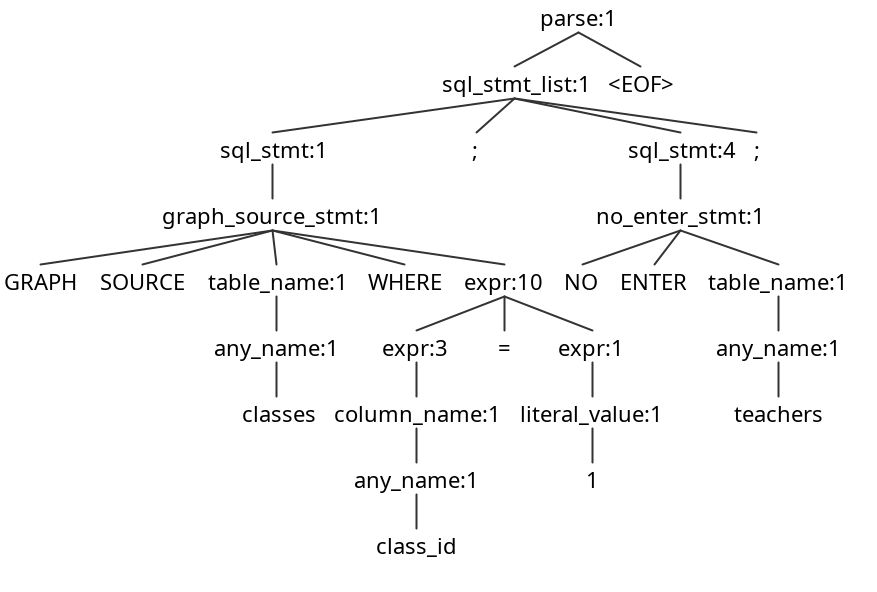
\includegraphics[scale=0.5]{./img/antlr4-parse-tree.png}
  \caption{Пример дерева синтаксического анализа}
  \label{antlr4-parse-tree}
\end{figure}

С использованием ANTLR4 на языке Python был сгенерирован синтаксический анализатор. Кроме того, была разработана программа, демонстрирующая возможности использования объектов ANTLR4.

Обход синтаксического дерева производится с использованием объекта ANTLR Слушатель (Listener), что позволяет реализовать соответствующую логику обработки для каждой конструкции. На рисунке \ref{antlr4-program} представлен код обработки конструкций \textit{GRAPH SOURCE} и \textit{NO ENTER}, который подразумевает простое отображение содержимого токенов. На рисунке \ref{antlr4-program-out} представлен вывод данной программы, соответствующий примеру метаданных, изображённым на рисунке \ref{metadata-example-4}.

\begin{figure}
  \begin{lstlisting}[language=Python]
from antlr4 import FileStream, CommonTokenStream, ParseTreeWalker
from RelatioLangLexer import RelatioLangLexer
from RelatioLangParser import RelatioLangParser
from RelatioLangParserListener import RelatioLangParserListener
from tools import get_original_token_text

class RelatioLangListener(RelatioLangParserListener):
    def exitGraph_source_stmt(self, ctx:RelatioLangParser.Graph_source_stmtContext):
        print("GRAPH SOURCE:")
        print(f"\ttable is \"{ctx.table_name().getText()}\"")
        if ctx.expr() is not None:
            print(f"\twhere statement is \"{get_original_token_text(ctx.expr())}\"")

    def exitNo_enter_stmt(self, ctx:RelatioLangParser.No_enter_stmtContext):
        print("NO ENTER:")
        print(f"\ttable is \"{ctx.table_name().getText()}\"")

def main():
    filename = input()
    input_stream = FileStream(filename)
    lexer = RelatioLangLexer(input_stream)
    stream = CommonTokenStream(lexer)
    parser = RelatioLangParser(stream)
    tree = parser.parse()
    relatio_lang_listiner = RelatioLangListener()
    walker = ParseTreeWalker()
    walker.walk(relatio_lang_listiner, tree)
  \end{lstlisting}
  \caption{Код c логикой обработки конструкций GRAPH SOURCE и NO ENTER}
  \label{antlr4-program}
\end{figure}

\begin{figure}
  \begin{lstlisting}
GRAPH SOURCE:
        table is "classes"
        where statement is "class_id=1"

NO ENTER:
        table is "teachers"
  \end{lstlisting}
  \caption{Пример работы программы, обрабатывающей конструкции}
  \label{antlr4-program-out}
\end{figure}

Использование ANTLR4 для генерации синтаксического анализатора демонстрирует его эффективность в разборе и обработке грамматических конструкций. Такой подход не только упрощает процесс разработки грамматик, но и предоставляет гибкие возможности для расширения логики обработки, что позволяет интегрировать более сложные структуры и правила в дальнейшем.
